Fig.(\ref{fig:gantt}) shows an approximate schedule for the next 12 months. In the following, each item is described in more detail.
\begin{figure}[hp]
\centering
\fbox{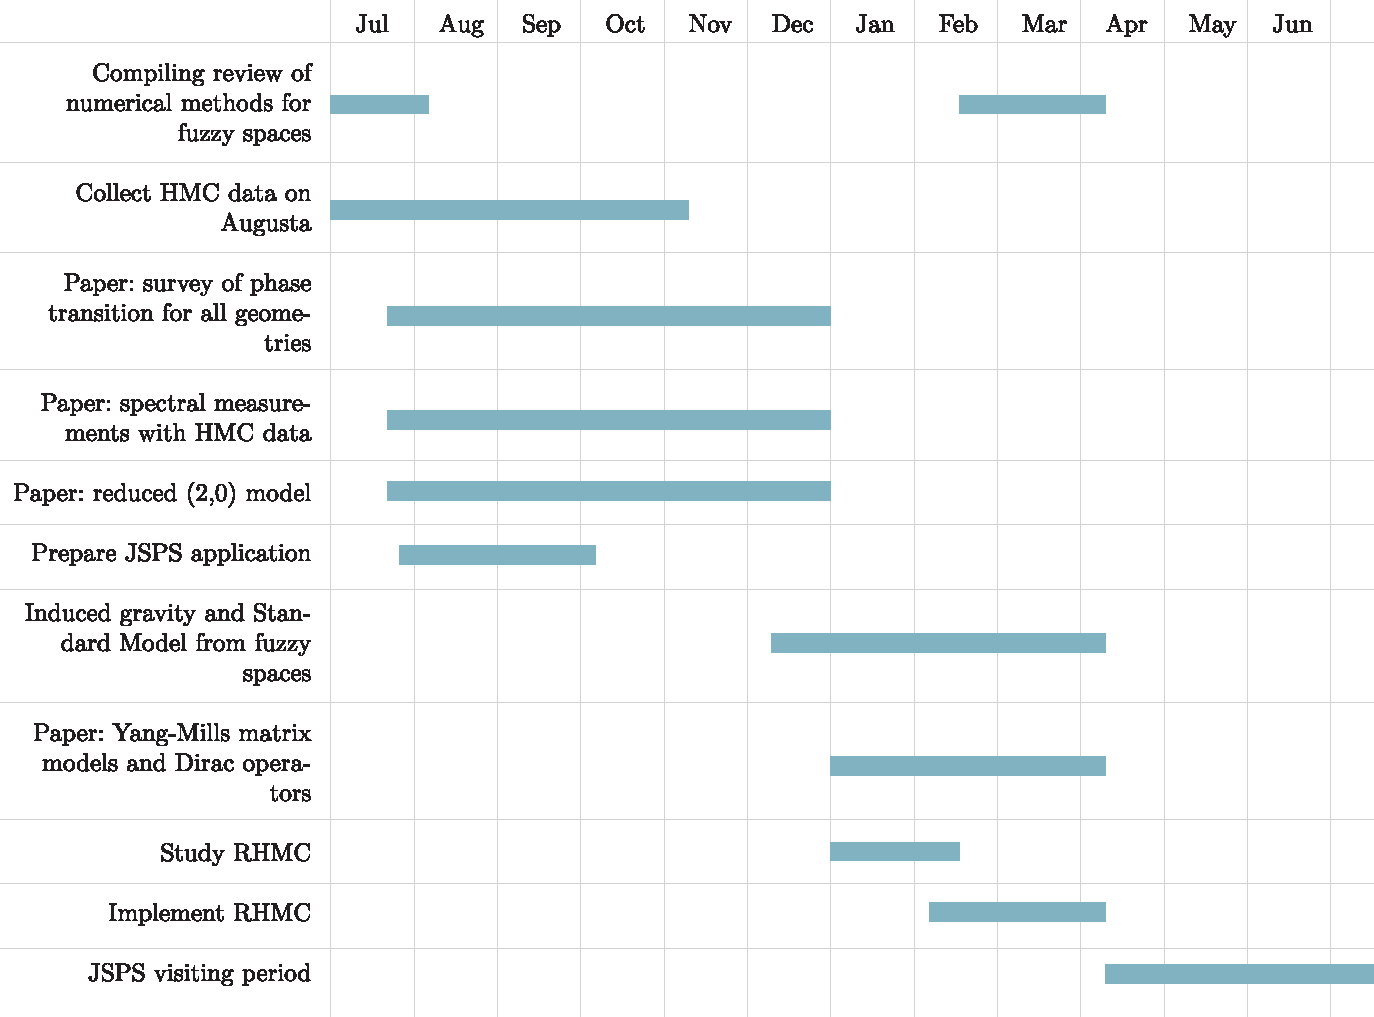
\includegraphics[angle=90,origin=c,width=1\linewidth]{fig/gantt.pdf}}
\caption{12-month Gantt chart}
\label{fig:gantt}
\end{figure}
\begin{enumerate}
\item \textit{Compiling review of numerical methods for fuzzy spaces}\newline
During the first two years of PhD a number of formulas and techniques were developed for an efficient implementation of Monte Carlo simulations of fuzzy spaces. Part of these have been coincisely included in the first and second year report. The goal is to collect them in a unique and coherent document that will constitute one chapter of the thesis.
\item \textit{Collect HMC data on Augusta}\newline
The new Hybrid Monte Carlo code presented in section (\ref{numimprov}) will allow to run simulations with larger matrices and better quality samples. Arrangements with the IT team are being made for running the code on the University of Nottingham high performance computing facility, Augusta. Since the code requires very little manual tuning, data will be collected hopefully almost non-stop in the next few months. 
\item \textit{Paper: survey of phase transition for all geometries}\newline
Phase transitions for some geometries have been studied in \cite{barrettglaser} and \cite{glaser}, but a systematic study is still lacking. The new data collected on Augusta should allow a precise characterization of the phase transition (critical coupling and critical exponents) for all $(p,q)$ geometries with $p+q = 2,3,4$ by means of finite-size scaling. An ansatz for a renormalization group approach to the study of phase transitions was briefly considered in the past but yielded unclear results; its use would require further refinement probably not achievable in the time frame proposed in the chart.
\item \textit{Paper: spectral measurements with better data}\newline
Recently some techniques were developed in \cite{barrdruceglaser} in an attempt to translate classical notions such as dimension or volume in the context of fuzzy spaces using spectral data. A preliminary study on random fuzzy spaces was also included for rather small matrices. An interesting test for these tools and the random fuzzy spaces program would be to study larger matrices and more geometries. However, it is not clear yet how the averaging process over Dirac operators should be implemented for these measurements (whether before or after extracting the dimension spectrum for example). 
\item \textit{Paper: reduced $(2,0)$ model}\newline
The results presented in section (\ref{sven}) are still partial and a useful reduced model has not been found yet. Ideally, the model should be able to describe the asymptotics on either side of the phase transition. This project will be developed further in the next few months under the supervision of Professor Sven Gnutzmann.
\item \textit{Prepare JSPS application / JSPS visiting period}\newline
The Japan Society for the Promotion of Science (JSPS) assigns a number of fellowships each year for a short-term visiting period in a host institution in Japan. The next application deadline is set for October 4 2019, with the visiting period starting anywhere between April 1 2020 and March 31 2021. Although no arrangements have been made yet, the plan would be to work with Professor Jun Nishimura at KEK on numerical simulations of the IKKT model \cite{ikkt}. Recently, some promising analytical results have been obtained in the model \cite{haroldCOSM}, while numerical methods have been developed to simulate the model in Lorentzian signature \cite{nishi}. The purpose of the visiting period would therefore be two-fold, as a first-hand experience of the model per se, and an opportunity to learn numerical techniques directly transferrable to fuzzy Dirac operators. 
\item \textit{Paper: Yang-Mills matrix models and Dirac operators}\newline
The link between Dirac operators and Yang-Mills matrix models is especially interesting in light of the aforementioned results on the IKKT model. The calculation presented in section (\ref{ymdo}) can be extended to the complete type $(0,3)$ Dirac operator, and the study be complemented with numerical results from the simulations. The chosen time frame would make the project a useful warm-up in the eventuality of being awarded the JSPS fellowship. 
\item \textit{Induced gravity and Standard Model from fuzzy spaces/ Study RHMC / implement RHMC}\newline
The matrix model analyzed so far should ideally describe a non-commutative analogue of a space-time manifold in a finite theory of quantum gravity. A number of results are being collected in support of this claim, the latest being the aforementioned spectral estimators for dimension and volume \cite{barrdruceglaser} and still unpublished results on the Lie algebraic structures that emerge among the matrices of certain models.\newline
A rather unsatisfactory aspect of the model is that no matter fields have entered the picture yet. A priori there is no guarantee that the model without matter should even be of physical relevance, and the presence of matter could produce dramatic deviations from the behaviour observed so far.\newline
The proposal for the introduction of matter fields is in the spirit of Sakharov's work on induced gravity \cite{sak}, and represents a possible final step in a progression that started in the early days of non-commutative geometry applied to the Standard Model. In \cite{connesGRAVMAT} Connes showed that there is no need to introduce gauge fields explicitly in the spectral action, as the bosonic sector of the Standard Model emerges naturally from inner fluctuations of the Dirac operator. Schematically, the spectral action Connes considered had the following form:
\begin{equation}
S = \Tr \chi \left( \frac{D}{\Lambda} \right) + \langle \Psi, D \Psi \rangle
\end{equation}
where the first term would produce the Einstein-Hilbert action plus the gauge and Higgs sector, and the second would produce the couplings between gauge fields and matter. Later on, in \cite{barrettIND} it was observed that Sakharov's mechanism could take care of the whole bosonic sector (gauge fields plus gravity), and a simpler action was proposed:
\begin{equation}\label{eq:ferac}
S = \langle \Psi, D \Psi \rangle.
\end{equation}
At this point space-time is still a commutative classical manifold $M$. By analogy, the natural way to introduce matter in the context of fuzzy spaces is to replace the manifold with a fuzzy space while keeping the same action (\ref{eq:ferac}). Grassmann integration over the fermions yields a determinant, therefore a convergency term in the action of the type $\Tr D^{2p}$ is needed as well. The simplest choice would then be:
\begin{equation}
S = g_2 \Tr D^2 - \frac{1}{2} \Tr \log D^2
\end{equation}
where the determinant has been expressed as a trace log.\newline
The inclusion of fermions entails both a theoretical and a numerical aspect. On the theoretical side, one might carry out explicitly the calculation of the action and identify the gravity, gauge and matter sectors of the theory. On the numerical side, a Monte Carlo simulation with a fermion determinant can be perfomed in various ways, the state of the art being an extension of HMC called Rational Hybrid Monte Carlo (RHMC) \cite{rhmc}.
\end{enumerate}